\chapter{Casi d'suo}
I casi d'uso permettono di modellare il comportamento del sistema e descrivere i requisiti funzionali in linguaggio naturale. Grazie a questi modelli è quindi possibile rappresentare il comportamento esterno del sistema, visto come una black-box, dal punto di vista di un'attore.

Oltre a una descrizione testuale (gli \emph{Scenari}) i casi d'uso possono esser rappresentati mediante diagrammi. In tali diagrammi troviamo le segunti entità:
 \begin{itemize}
  \item gli attori: essi rappresentano un soggetto o un'entità esterna che interagisce col sistema
  \item i casi d'uso: rappresentano un particolare scenario di interazione tra attore e sistema. Sono rappresentati graficamente da ellissi
  \item le associazioni: rappresentate da una linea mettono in comunicazione un attore con i caso d'uso
 \end{itemize}

 Nei prossimi paragrafi saranno mostrati alcuni dei casi d'uso modellati durante la fase di analisi.
 \newpage
 
 \section{Diagrammi dei casi d'uso}
 
 \subsection{Caso d'uso: Ricarica telefonica}
	\begin{figure}[!htbp]
	  \centering
	  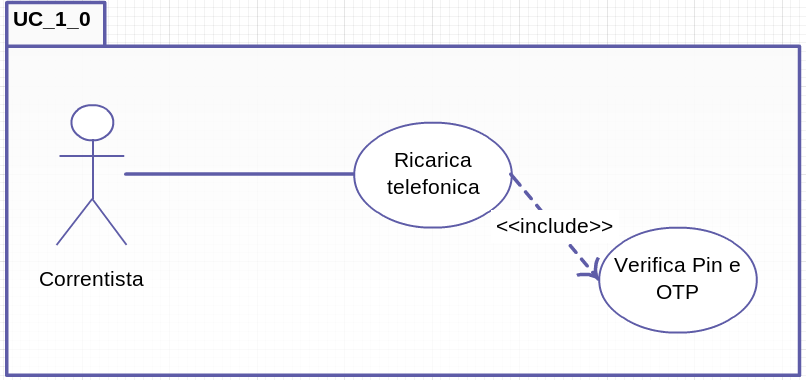
\includegraphics[scale=0.65]{casi_uso/ricarica.png}
	\end{figure}
	
  \subsection{Caso d'uso: Ricarica telefonica}
 	\begin{figure}[!htbp]
	  \centering
	  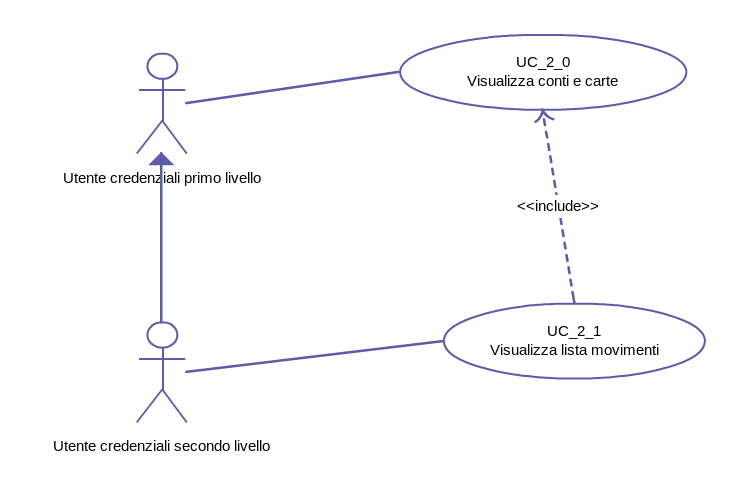
\includegraphics[scale=0.65]{casi_uso/conti.png}
	\end{figure}
	

 \section{Specifica dei casi d'uso}
 
 \subsection{Caso d'uso: Ricarica telefonica}

 Le tabelle \ref{tab:uc1}, \ref{tab:uc2}, \ref{tab:uc3}, \ref{tab:uc4}, \ref{tab:uc5} mostrano i casi d'uso relativi all'operazione di ricarica telefonica, nel caso in cui l'utente decida di ricaricare un numero di telefono associato ad un contatto presente nella rubrica del dispositivo.
 
 
\begin{center}
    \captionof{table}{Caso d'uso ricarica telefonica}
    \label{tab:uc1}
     \begin{longtable}{{ | l | p{8cm} |}}
    \hline
    \textbf{Caso d'uso} UC\_1\_0 & Ricarica telefonica di un numero salvato in rubrica \\ \hline
    \textbf{Attore} & Correntista bancario  \\ \hline
    \textbf{Precondizioni} & L'utente è loggato al sistema e ha iniziato una sessione inserendo un codice OTP  \\ \hline
    \textbf{Postcondizioni di successo}  & Il sistema ha registrato l'operazione \\\hline
    \textbf{Postcondizioni di fallimento}   &  Il sistema non ha registrato l'operazione\\\hline
    \textbf{Scenario} &  \\\hline
    & \begin{enumerate}
       \item L'utente seleziona l'operazione di ricarica telefonica \label{item:sel8}
       \item \texttt{Include} UC\_1\_1 \emph{Visualizza lista beneficiari}
       \item \texttt{Include} UC\_1\_2 \emph{Visualizza lista conti di addebito}
       \item \texttt{Include} UC\_1\_3 \emph{Visualizza lista operatori}
       \item \texttt{Include} UC\_1\_4 \emph{Verifica pin e OTP}
       
%        \item \label{item:sel1}Il sistema visualizza l'elenco dei beneficiari
%        \item L'utente seleziona un beneficiario 
%        \item \label{item:sel2}Il sistema visualizza l'elenco dei conti per l'addebbito
%        \item L'utente seleziona un conto
%        \item \label{item:sel3}\label{item:compagnia} Il sistema mostra l'elenco delle compagnie telefoniche
%        \item L'utente seleziona una compagnia telefonica
%        \item \label{item:sel4}Il sistema visualizza i tagli disponibili
%        \item L'utente seleziona un taglio di ricarica
%        \item \label{item:sel5}\label{item:beneficiario} Il sistema mostra il riepilogo dell'operazione e richiede conferma
%        \item L'utente conferma i dati
%        \item \label{item:credenziali}\label{item:sel6}Il sistema richiede Pin e OTP
%        \item L'utente immette i dati richiesti e conferma
%        \item \texttt{Include} \emph{Verifica credenziali}
       \item Il sistema mostra lo scontrino dell'operazione
      \end{enumerate}\\\hline
      \textbf{Scenari alternativi} &  \\\hline
     & \begin{itemize}
       \item  \ref{item:sel8} L'utente annulla operazione
       \item Il caso d'uso termina
      \end{itemize}\\\hline
     \end{longtable}
\end{center}

\begin{center}   
    \captionof{table}{Caso d'uso selezione beneficiario}
    \label{tab:uc2}
     \begin{longtable}{{ | l | p{8cm} |}}
    \hline
    \textbf{Caso d'uso} UC\_1\_1 & Selezione beneficiario \\ \hline
    \textbf{Attore} & Correntista bancario  \\ \hline
    \textbf{Precondizioni} & L'utente ha iniziato una nuova ricarica telefonica \\ \hline
    \textbf{Postcondizioni di successo}  & Il sistema ha convalidato la scelta del beneficiario \\\hline
    \textbf{Postcondizioni di fallimento}   &  Il sistema non ha cambiato stato\\\hline
    \textbf{Scenario} &  \\\hline
    & \begin{enumerate}
       \item \label{item:beneficiario} Il sistema visualizza la lista dei beneficiari
       \item L'utente seleziona un beneficiario 
       \item Il sistema aggiorna l'interfaccia con la selezione effettuata 
      \end{enumerate}\\\hline
      \textbf{Scenari alternativi} &  \\\hline
    & \begin{enumerate}
    \setcounter{enumi}{1}
       \item L'utente seleziona la voce \emph{Beneficiario}
       \item Il caso d'uso riprende dal punto \ref{item:beneficiario}
      \end{enumerate}\\\hline
     & \begin{itemize}
       \item L'utente annulla l'operazione
       \item Il caso d'uso termina
      \end{itemize}\\\hline

     \end{longtable}
\end{center}

\begin{center}
    \captionof{table}{Caso d'uso selezione conto di addebito}
    \label{tab:uc3}
     \begin{longtable}{{ | l | p{8cm} |}}
    \hline
    \textbf{Caso d'uso} UC\_1\_2 & Selezione conto di addebito \\ \hline
    \textbf{Attore} & Correntista bancario  \\ \hline
    \textbf{Precondizioni} & L'utente ha iniziato una nuova ricarica telefonica \\ \hline
    \textbf{Postcondizioni di successo}  & Il sistema ha convalidato la scelta del conto \\\hline
    \textbf{Postcondizioni di fallimento}   &  Il sistema non ha cambiato stato\\\hline
    \textbf{Scenario} &  \\\hline
    & \begin{enumerate}
       \item \label{item:conto} Il sistema visualizza la lista dei conti disponibili
       \item L'utente seleziona un conto 
       \item Il sistema aggiorna l'interfaccia con la selezione effettuata 
      \end{enumerate}\\\hline
      \textbf{Scenari alternativi} &  \\\hline
    & \begin{enumerate}
    \setcounter{enumi}{1}
       \item L'utente seleziona la voce \emph{Conto di addebito}
       \item Il caso d'uso riprende dal punto \ref{item:conto}
      \end{enumerate}\\\hline
     & \begin{itemize}
       \item L'utente annulla l'operazione
       \item Il caso d'uso termina
      \end{itemize}\\\hline
     \end{longtable}
\end{center}

\begin{center}
    \captionof{table}{Caso d'uso selezione operatore}
    \label{tab:uc4}
     \begin{longtable}{{ | l | p{8cm} |}}
    \hline
    \textbf{Caso d'uso} UC\_1\_3 & Selezione operatore \\ \hline
    \textbf{Attore} & Correntista bancario  \\ \hline
    \textbf{Precondizioni} & L'utente ha iniziato una nuova ricarica telefonica \\ \hline
    \textbf{Postcondizioni di successo}  & Il sistema ha convalidato la scelta dell'operatore \\\hline
    \textbf{Postcondizioni di fallimento}   &  Il sistema non ha cambiato stato\\\hline
    \textbf{Scenario} &  \\\hline
    & \begin{enumerate}
       \item \label{item:compagnia}Il sistema visualizza la lista delle compagnie telefoniche
       \item L'utente seleziona una compagnia 
       \item \label{item:tagli} Il sistema mostra i tagli di ricarica disponibili
       \item L'utente seleziona un taglio di ricarica
       \item Il sistema aggiorna l'interfaccia con la selezione effettuata
      \end{enumerate}\\\hline
      \textbf{Scenari alternativi} &  \\\hline
    & \begin{enumerate}
    \setcounter{enumi}{1}
       \item L'utente seleziona la voce \emph{Importo}
       \item Il caso d'uso riprende dal punto \ref{item:tagli}
      \end{enumerate}\\\hline
     & \begin{itemize}
       \item L'utente annulla l'operazione
       \item Il caso d'uso termina
      \end{itemize}\\\hline
    \textbf{Scenari di errore} &  \\\hline
    & \begin{enumerate}
    \setcounter{enumi}{1}
       \item L'utente seleziona una compagnia telefonica errata
       \item Il sistema mostra messaggio di errore
       \item Il caso d'uso riprende dal punto \ref{item:compagnia}
      \end{enumerate}\\\hline

     \end{longtable}
\end{center}

\begin{center}
    \captionof{table}{Caso d'uso verifica Pin e OTP}
    \label{tab:uc5}
     \begin{longtable}{{ | l | p{8cm} |}}
    \hline
    \textbf{Caso d'uso} UC\_1\_4 & Verifica Pin e OTP \\ \hline
    \textbf{Attore} & Correntista bancario  \\ \hline
    \textbf{Precondizioni} & L'utente ha iniziato una nuova ricarica telefonica e ha immesso tutti i dati richiesti\\ \hline
    \textbf{Postcondizioni di successo}  & Il sistema ha convalidato l'operazione e ha aggiornato il suo stato \\\hline
    \textbf{Postcondizioni di fallimento}   &  Il sistema non ha convalidato l'operazione e ha mostrato un messaggio di errore\\\hline
    \textbf{Scenario} &  \\\hline
    & \begin{enumerate}
       \item  Il sistema mostra il riepilogo dell'operazione e richiede conferma
       \item L'utente conferma i dati
       \item \label{item:credenziali}Il sistema richiede Pin e OTP
       \item L'utente immette i dati richiesti e conferma
       \item Il sistema verifica le credenziali
       \item Il sistema mostra lo scontrino dell'operazione effettuata
     \end{enumerate}\\\hline
      \textbf{Scenari alternativi} &  \\\hline
     & \begin{itemize}
       \item L'utente annulla l'operazione
       \item Il caso d'uso termina
      \end{itemize}\\\hline
     & \begin{enumerate}
      \setcounter{enumi}{4}
       \item Il sistema non valida le credenziali
       \item Il sistema visualizza tipo il di errore
       \item Il caso d'uso riprende dal punto \ref{item:credenziali}
      \end{enumerate}\\\hline
     \end{longtable}
\end{center}

 \subsection{Caso d'uso: Visualizza lista conti e carte e Visualizza lista movimenti}

\begin{center}
    \captionof{table}{Caso d'uso visualizza conti e carte}
    \label{tab:uc6}
     \begin{longtable}{{ | l | p{8cm} |}}
    \hline
    \textbf{Caso d'uso} & UC\_2\_0  Visualizza lista conti e carte \\ \hline
    \textbf{Attore} & Correntista bancario  \\ \hline
    \textbf{Precondizioni} & L'utente ha effettuato un login di primo o secondo livello \\ \hline
    \textbf{Postcondizioni di successo}  & Il sistema rimane nel suo stato o aggiorna la lista dei conti in memoria \\\hline
    \textbf{Postcondizioni di fallimento}   &  Il sistema rimane nel suo stato\\\hline
    \textbf{Scenario} &  \\\hline
    & \begin{enumerate}
       \item L'utente seleziona l'operazione di visualizzazione lista conti e carte
       \item \label{item:verificalista}Il sistema verifica che l'elenco dei prodotti non è vuoto
       \item Il sistema mostra la lista dei prodotti
      \end{enumerate}\\\hline
    \textbf{Scenario alternativo} &  \\\hline
    & \begin{enumerate}
    \setcounter{enumi}{1}
       \item Il sistema ha verificato che la lista dei prodotti è vuota
       \item Il sistema notifica l'evento con un opportuno messaggio
	\item Il caso d'uso termina
       \end{enumerate}\\\hline
    \textbf{Scenario di errore} &  \\\hline
    & \begin{enumerate}
    \setcounter{enumi}{1}
       \item Il sistema riceve un errore
       \item Il sistema notifica l'evento con un messaggio di errore e la possibilità di riprovare l'azione
       \item L'utente seleziona \emph{riprova}
       \item Il caso d'uso riprende dal punto \ref{item:verificalista}
       \end{enumerate}\\\hline
     \end{longtable}
\end{center}

\begin{center}
    \captionof{table}{Caso d'uso visualizza lista movimenti}
    \label{tab:uc7}
     \begin{longtable}{{ | l | p{8cm} |}}
    \hline
    \textbf{Caso d'uso} & UC\_2\_1  Visualizza lista movimenti \\ \hline
    \textbf{Attore} & Correntista bancario  \\ \hline
    \textbf{Precondizioni} & L'utente ha effettuato un login di secondo livello \\ \hline
    \textbf{Postcondizioni di successo}  & Il sistema rimane nel suo stato \\\hline
    \textbf{Postcondizioni di fallimento}   &  Il sistema rimane nel suo stato\\\hline
    \textbf{Scenario} &  \\\hline
    & \begin{enumerate}
       \item \texttt{Include} UC\_2\_0 \emph{Visualizza lista conti e carte}
       \item L'utente seleziona un conto o una carta
       \item \label{item:verificamovimenti}Il sistema verifica che la lista dei movimenti non è vuoto
       \item Il sistema mostra la lista dei prodotti
      \end{enumerate}\\\hline
    \textbf{Scenario alternativo} &  \\\hline
    & \begin{enumerate}
    \setcounter{enumi}{1}
       \item Il sistema ha verificato che la lista dei movimenti è vuota
       \item Il sistema notifica l'evento con un opportuno messaggio
	\item \texttt{Extend} \emph{Filtra movimenti per data}
       \end{enumerate}\\\hline
    \textbf{Scenario di errore} &  \\\hline
    & \begin{enumerate}
    \setcounter{enumi}{1}
       \item Il sistema riceve un errore
       \item Il sistema notifica l'evento con un messaggio di errore e la possibilità di riprovare l'azione
       \item L'utente seleziona \emph{riprova}
       \item Il caso d'uso riprende dal punto \ref{item:verificamovimenti}
       \end{enumerate}\\\hline
     \end{longtable}
\end{center}
